\documentclass{fmbvecto}

\usepackage[spanish]{babel}
\usepackage{caption}

\renewcommand{\title}{Ejemplo de solución correcta del taller 3}
\newcommand{\subject}{Cálculo Vectorial}

\renewcommand{\labelenumii}{\theenumii}
\renewcommand{\theenumii}{\theenumi.\arabic{enumii}.}

\NewDocumentCommand{\itemp}{o}{\item (#1 puntos)}


\begin{document}

Miércoles, 24 de julio de 2024

\begin{center}
    \textbf{\LARGE \title} \\
    {\large \subject}
\end{center}


Profesor: Jacinto Eloy Puig Portal, \href{mailto:jpuig@uniandes.edu.co}{jpuig@uniandes.edu.co}. \\
Monitor: Federico Melo Barrero, \href{mailto:f.melo@uniandes.edu.co}{f.melo@uniandes.edu.co}.\\

\textbf{\Large Preámbulo}

Las instrucciones referentes a la entrega del taller están escritas en \href{https://bloqueneon.uniandes.edu.co/d2l/home}{Bloque Neón}.

\subsection*{Indicación}

Resuelva únicamente un ejercicio de cada sección. Si resuelve más de uno, se calificará alguno arbitrariamente.

\subsection*{Bonos}
\begin{itemize}
  \item Se sumarán 0.25 puntos de bonificación a la nota del taller si su contenido está ordenado y puede leerse con facilidad.
  \item Se sumarán 0.25 puntos de bonificación a la nota del taller si no contiene errores léxicos, gramaticales ni faltas de ortografía.
\end{itemize}
La nota del taller puede exceder el 5.0.

\subsection*{Recomendaciones}

No necesita hacer uso de herramientas que le ayuden a hacer matemáticas, ya sean calculadoras, aplicaciones, grandes modelos de lenguaje u otras. Le recomiendo que no lo haga.

Recuerde incluir las unidades siempre que trate con magnitudes físicas.

\subsection*{Nota}

Dado que este es un ejemplo de solución correcta, se muestra la solución para un ejercicio por cada sección, en consonancia con las instrucciones dadas a los estudiantes. Recuerde que, en caso de que haya resuelto más de un ejercicio por sección, se calificará alguno arbitrariamente.

Esto es realmente tras ver la falta de acogida de los ejercicios teóricos, en particular de las dos demostraciones. En caso de deberse eso a restricciones de tiempo, les animo a abordarlas en la posteridad, con más calma, en aras de refinar su entendimiento matemático. Con eso en mente, en lugar de ofrecerles una solución tan detallada como acostumbro, en esos ejercicios les proveo un bosquejo de la solución. Una sugerencia, si se quiere.


\section{Taller 2}

\begin{problema}[Corrección del taller 2]
    
    (1.25 puntos) Corrija todos los errores que tuvo en el taller 2. Si no tuvo errores, omita este punto.

    \tcblower
    
    En este punto simplemente revisaré que se hayan corregido los errores y abordado los comentarios que dejé en su taller. Naturalmente, la corrección debe ser correcta, sobretodo teniendo en cuenta que el solucionario del taller 2 está en Bloque Neón desde el miércoles 10 de julio.

\end{problema}

\section{Teorema de Green}

\begin{problema}[Cálculo de integrales de línea con el teorema de Green]
    
    (1.25 puntos) Sea \(\bvec{F}\colon \mathbb{R}^2 \to \mathbb{R}^2\) el campo vectorial dado por
    \[
    \bvec{F}(x, y) = (\mathrm{e}^{-x} + y^2, \mathrm{e}^{-y} + x^2).
    \]
    y sea \(D\) una región cuya frontera consiste de la unión entre:
    \begin{itemize}
    \item El arco de la curva \(y = \cos x\) que abarca entre los puntos \(\left(-\frac{\uppi}{2}, 0\right)\) y \(\left(\frac{\uppi}{2}, 0\right)\).
    \item El segmento de recta que va desde \(\left(\frac{\uppi}{2}, 0\right)\) hasta \(\left(-\frac{\uppi}{2}, 0\right)\).
    \end{itemize}
    Calcule la integral de línea de \(\bvec{F}\) sobre \(\partial D\).

\tcblower
\textbf{Solución:}

    Primeramente, note que la región \(D\) se puede escribir formalmente (y más concisamente) como
    \[
    D = \left\{ (x, y) \in \mathbb{R}^2 \mid -\frac{\uppi}{2} \leq x \leq \frac{\uppi}{2} \ \land \ 0 \leq y \leq \cos x \right\}.
    \]
    Con eso en mente, realmente para solucionar este problema basta con utilizar directamente el teorema de Green. \(\partial D\) denota la frontera de la región \(D\), orientada positivamente por convención. Según el teorema de Green, la integral de línea sobre la frontera de una región es igual a la integral del rotacional del campo vectorial sobre la región:
    \begin{align*}
        \int_{\partial D} \bvec{F} \cdot \mathrm{d}\bvec{r} &= \iint_D \rot \bvec{F} \: \mathrm{d}A \\
        &= \iint_D \left( \frac{\partial F_2}{\partial x} - \frac{\partial F_1}{\partial y} \right) \: \mathrm{d}A \\
        &= \iint_D \left( \frac{\partial}{\partial x} (\mathrm{e}^{-y} + x^2) - \frac{\partial}{\partial y} (\mathrm{e}^{-x} + y^2) \right) \: \mathrm{d}A \\
        &= \iint_D \left( 2x - 2y \right) \: \mathrm{d}A.
    \end{align*}
    Lo anterior es una integral doble, como las que se han trabajado en talleres previos. Los límites se plantean según la descripción de la región \(D\) al inicio de la solución.
    \begin{align*}
        \iint_D \left( 2x - 2y \right) \: \mathrm{d}A &= \int_{-\frac{\uppi}{2}}^{\frac{\uppi}{2}} \int_0^{\cos x} \left( 2x - 2y \right) \: \mathrm{d}y \: \mathrm{d}x \\
        &= \int_{-\frac{\uppi}{2}}^{\frac{\uppi}{2}} \left[ 2xy - y^2 \right]_0^{\cos x} \: \mathrm{d}x \\
        &= \int_{-\frac{\uppi}{2}}^{\frac{\uppi}{2}} 2x \cos x - \cos^2 x \: \mathrm{d}x \\
        &= \int_{-\frac{\uppi}{2}}^{\frac{\uppi}{2}} 2x \cos x \: \mathrm{d}x - \int_{-\frac{\uppi}{2}}^{\frac{\uppi}{2}} \cos^2 x \: \mathrm{d}x \\
        &= I_1 - I_2.
    \end{align*}
    Se resuelve primero la integral \(I_1\), empleando integración por partes. Se toma \(u = x\) y \(\mathrm{d}v = \cos x \: \mathrm{d}x\), de forma que \(\mathrm{d}u = \mathrm{d}x\) y \(v = \sin x\). Se tiene entonces
    \begin{align*}
        I_1 &= \left[ x \sin x \right]_{-\frac{\uppi}{2}}^{\frac{\uppi}{2}} - \int_{-\frac{\uppi}{2}}^{\frac{\uppi}{2}} \sin x \: \mathrm{d}x \\
        &= \left( \frac{\uppi}{2} \sin \left(\frac{\uppi}{2}\right) - \left( -\frac{\uppi}{2} \sin \left(-\frac{\uppi}{2}\right) \right) \right) - \left[ -\cos x \right]_{-\frac{\uppi}{2}}^{\frac{\uppi}{2}} \\
        &= \left( \frac{\uppi}{2} \sin \left(\frac{\uppi}{2}\right) - \left( -\frac{\uppi}{2} \sin \left(-\frac{\uppi}{2}\right) \right) \right) + \cos \left(\frac{\uppi}{2}\right) - \cos \left(-\frac{\uppi}{2}\right).
    \end{align*}
    Al computar los valores de las funciones trigonométricas, recuerde que \(\sin \frac{\uppi}{2} = 1\), \(\sin -\frac{\uppi}{2} = -1\), \(\cos \frac{\uppi}{2} = 0\) y \(\cos -\frac{\uppi}{2} = 0\). Esto lo puede comprobar fácilmente con la circunferencia unitaria. Por ende, se tiene que
    \begin{align*}
        I_1 &= \left( \frac{\uppi}{2} - \left( -\frac{\uppi}{2} \cdot -1 \right) \right) + 0 - 0 \\
        &= \uppi + \frac{\uppi}{2} \\
        &= 0.
    \end{align*}
    Ahora, para resolver la integral \(I_2\), se puede usar la identidad trigonométrica \(\cos^2 x = \frac{1 + \cos 2x}{2}\). Se tiene entonces
    \begin{align*}
        I_2 &= \int_{-\frac{\uppi}{2}}^{\frac{\uppi}{2}} \frac{1 + \cos 2x}{2} \: \mathrm{d}x \\
        &= \frac{1}{2} \int_{-\frac{\uppi}{2}}^{\frac{\uppi}{2}} 1 + \cos 2x \: \mathrm{d}x \\
        &= \frac{1}{2} \left[ x + \frac{1}{2} \sin 2x \right]_{-\frac{\uppi}{2}}^{\frac{\uppi}{2}} \\
        &= \frac{1}{2} \left( \frac{\uppi}{2} + \frac{1}{2} \sin \uppi - \left( -\frac{\uppi}{2} + \frac{1}{2} \sin \left(-\uppi\right) \right) \right) \\
        &= \frac{1}{2} \left( \frac{\uppi}{2} + \frac{1}{2} \cdot 0 - \left( -\frac{\uppi}{2} + \frac{1}{2} \cdot 0 \right) \right) \\
        &= \frac{1}{2} \left( \frac{\uppi}{2} + \frac{\uppi}{2} \right) \\
        &= \frac{\uppi}{2}.
    \end{align*}
    Por ende, la integral de línea de \(\bvec{F}\) sobre \(\partial D\) es
    \begin{align*}
        \int_{\partial D} \bvec{F} \cdot \mathrm{d}\bvec{r} &= I_1 - I_2 \\
        &= 0 - \frac{\uppi}{2} \\
        &= -\frac{\uppi}{2}.
    \end{align*}
    Se concluye entonces que:
    \begin{gbox}
        La integral de línea de \(\bvec{F}\) sobre \(\partial D\) es \(-\frac{\uppi}{2}\).
    \end{gbox}

\end{problema}

\phantom{}

\begin{problema}[Verificación de la fórmula de cambio de variables para integrales dobles]
    
    (1.25 puntos) Sírvase del teorema de Green para probar la fórmula de cambio de variables para integrales dobles en el caso particular en el que la función a transformar es \(1\). Ya debe estar familiarizado con ella, pero en caso contrario, la fórmula es la siguiente: 
    \[
    \iint_R \: \mathrm{d}x \: \mathrm{d}y = \iint_S \: \left| \frac{\partial(x, y)}{\partial(u, v)} \right| \: \mathrm{d}u \: \mathrm{d}v.
    \]

\tcblower
\textbf{Sugerencia para la solución:}\\

    Como digo en la nota en la parte de arriba, esto no constituye una solución al ejercicio, sino que es más bien una sugerencia que puede desatascarlo en caso de intentarlo en el futuro. \\
    
    A partir del teorema de Green, es posible establecer que 
    \[
    \iint_R \: \mathrm{d}x \: \mathrm{d}y = \int_{\partial R} x \: \mathrm{d}y.
    \]
    Allí, \(x = g(u, v)\) y \(\mathrm{d}y = \frac{\partial h}{\partial u} \: \mathrm{d}u + \frac{\partial h}{\partial v} \: \mathrm{d}v\). \\
    
    Eso se puede reemplazar en la integral y expandir, luego usar el teorema de Green para llevar la integral de vuelta a una integral doble y tras eso es cuestión de manipular los términos para demostrar la propiedad.
\end{problema}

\section{Teorema de Stokes}

\begin{problema}[Cálculo de integrales de superficie con el teorema de Stokes]
    
    (1.25 puntos) Sea \(\bvec{F}\colon \mathbb{R}^3 \to \mathbb{R}^3\) el campo vectorial dado por
    \[
    \bvec{F}(x, y, z) = (xyz, xy, x^2yz).
    \]
    y sea \(S\) la superficie que consiste de la cara de arriba y las cuatro caras laterales de un cubo de lado \(2\) centrado en el origen, con caras paralelas a los planos coordenados y orientada hacia afuera. Calcule la integral de superficie de \(\rot \bvec{F}\) sobre \(S\).

\tcblower
\textbf{Solución:}\\

    Se busca la integral de superficie de \(\rot \bvec{F}\) sobre \(S\). Se sabe que una forma de evitar evaluar la integral de superficie directamente es aplicar el teorema de Stokes, que relaciona la integral de línea de un campo vectorial sobre la frontera de una superficie con la integral de superficie del rotacional del campo vectorial sobre la superficie:
    \[
    \int_{\partial S} \bvec{F} \cdot \mathrm{d}\bvec{r} = \iint_S \rot \bvec{F} \cdot \mathrm{d}\bvec{S}.
    \]
    Con eso en mente, se quiere determinar la frontera de  \(S\). Note que la superficie \(S\) es el cubo con vértices en \((\pm 1, \pm 1, \pm 1)\) sin la cara de abajo, que es el cuadrado en el plano \(z = -1\). Por ende, una curva que actúa como borde de la superficie \(S\), \(\partial S\), es precisamente el perímetro de ese cuadrado en el plano \(z = -1\). Para que esté orientado positivamente, se recorre en sentido contrario a las manecillas del reloj visto desde arriba, como se muestra en la figura \ref{fig:cubo}.

    \begin{center}
    \includegraphics[width=0.7\textwidth]{stokes.jpeg}
    \captionof{figure}{Se usa el teorema de Stokes dos veces para transformar la integral.}
    \label{fig:cubo}
    \end{center}
    \vspace*{1em}

    Ahora, antes de precipitarse a evaluar la integral de línea sobre \(\partial S\), vale la pena contemplar la otra superficie delimitada por \(\partial S\): el cuadrado en el plano \(z = -1\). Se muestra también en la \ref{fig:cubo}. Si se orienta ese cuadrado de forma que coincida con la orientación positiva de \(\partial S\), se puede aplicar nuevamente el teorema de Stokes, ahora pasando de una integral de línea a otra integral de superficie, para integrar sobre ese cuadrado, obteniendo una integral más sencilla. Para ello, al orientar el cuadrado, se debe elegir como vector normal a la superficie algún vector paralelo a \(\uvec{k}\).\\
    
    Formalmente, denoto por \(\hat{S}\) a la superficie delimitada por \(\partial S\) en el plano \(z = -1\), de forma que
    \[
        \hat{S} = \left\{ (x, y, -1) \in \mathbb{R}^3 \mid -1 \leq x \leq 1 \ \land \ -1 \leq y \leq 1 \right\}.
    \]
    aplicando el teorema de Stokes según el raciocinio expuesto arriba, se tiene que
    \[
    \int_{\partial S} \bvec{F} \cdot \mathrm{d}\bvec{r} = \iint_S \rot \bvec{F} \cdot \mathrm{d}\bvec{S} = \iint_{\hat{S}} \rot \bvec{F} \cdot \mathrm{d}\bvec{S}.
    \]
    donde la integral más sencilla de evaluar es la última. A continuación se procede a calcularla. Primero, se calcula el rotacional de \(\bvec{F}\):
    \begin{align*}
        \rot \bvec{F} &= \nabla \times \bvec{F} \\
        &= \begin{vmatrix}
            \uvec{i} & \uvec{j} & \uvec{k} \\
            \frac{\partial}{\partial x} & \frac{\partial}{\partial y} & \frac{\partial}{\partial z} \\
            xyz & xy & x^2yz
        \end{vmatrix} \\
        &= \left( \frac{\partial}{\partial y} (x^2yz) - \frac{\partial}{\partial z} (xy), \frac{\partial}{\partial z} (xyz) - \frac{\partial}{\partial x} (x^2yz), \frac{\partial}{\partial x} (xy) - \frac{\partial}{\partial y} (xyz) \right) \\
        &= (x^2z, xy-2xyz, y-xz).
    \end{align*}
    Luego, para la integral de superficie, será necesario calcular el producto punto de \(\rot \bvec{F}\) con el vector normal a \(\hat{S}\), que es \(\uvec{k}\). Se computa dicho producto punto
    \begin{align*}
        \rot \bvec{F} \cdot \bvec{n} &= (x^2z, xy-2xyz, y-xz) \cdot \uvec{k} \\
        &= (x^2z, xy-2xyz, y-xz) \cdot (0, 0, 1) \\
        &= y-xz.
    \end{align*}
    Por la descripción de la superficie \(\hat{S}\), sabemos que \(z = -1\), por lo que el producto punto se simplifica a \(y+x\). Se reemplaza eso en la integral de superficie, donde los límites de integración se colocan tal y como están en la descripción del conjunto \(\hat{S}\):
    \begin{align*}
        \iint_{\hat{S}} \rot \bvec{F} \cdot \mathrm{d}\bvec{S} &= \iint_{\hat{S}} \rot \bvec{F} \cdot \bvec{n} \: \mathrm{d}S \\
        &= \int_{-1}^1 \int_{-1}^1 (x + y) \: \mathrm{d}x \: \mathrm{d}y \\
        &= \int_{-1}^1 \left[ \frac{x^2}{2} + xy \right]_{-1}^1 \: \mathrm{d}y \\
        &= \int_{-1}^1 \frac{1}{2} + y - \frac{1}{2} + y \: \mathrm{d}y \\
        &= \int_{-1}^1 2y \: \mathrm{d}y \\
        &= \left[ y^2 \right]_{-1}^1 \\
        &= 1^2 - (-1)^2 \\
        &= 1 - 1 \\
        &= 0.
    \end{align*}

    Con eso se ha arribado a la solución del problema:
    \begin{gbox}
        La integral de superficie de \(\rot \bvec{F}\) sobre \(S\) es \(0\).
    \end{gbox}
\end{problema}

\phantom{}

\begin{problema}[Propiedad de la integral de línea y la integral de superficie]
    
    (1.25 puntos) Demuestre o refute que 
    \[
    \int_C (f \nabla g) \cdot \mathrm{d}\bvec{r} = \iint_S (\nabla f \times \nabla g) \cdot \mathrm{d}S,
    \]
    donde \(C\) es una curva cerrada simple y suave, \(S\) es una superficie cerrada simple y suave, y \(f, g\) son funciones escalares de clase \(C^2\).

\tcblower
\textbf{Sugerencia para la solución:}\\

    Note que en el enunciado de la propiedad, en ningún momento se traza un vínculo entre la curva \(C\) y la superficie \(S\). En particular, sería errado presumir que \(C = \partial S\) para intentar aplicar el teorema de Stokes. Si eso fuera verdad, la propiedad sería verdadera; sin esa condición, la propiedad carece de sentido. \\
    
    Para convercerse de que la propiedad es falsa y refutarla, basta con tomar un contraejemplo. Hago hincapié en que puede tomar cualquier curva cerrada simple y suave \(C\) y cualquier superficie cerrada simple y suave \(S\). Similarmente, puede elegir cualesquiera funciones escalares \(f\) y \(g\), mientras sean de clase \(C^2\).\\

    Mientras elija una curva y una superficie que no tengan relación alguna, es extremadamente improbable que obtenga una igualdad, con lo cual exitosamente refutará la propiedad.

\end{problema}

\section{Teorema de Gauss}

\begin{problema}[Interpretación geométrica del teorema de Gauss]
    
    (1.25 puntos) Considere el campo vectorial graficado en la figura \ref{fig:vector-field}. Sírvase de la interpretación geométrica del teorema de Gauss para determinar el signo de la divergencia del campo en cada uno de los puntos resaltados.

    \begin{center}
    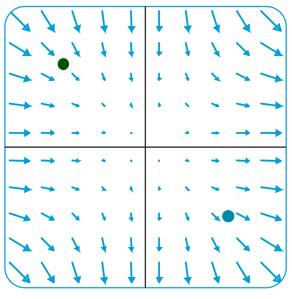
\includegraphics[width=0.4\textwidth]{vector-field.png}
    \captionof{figure}{Campo vectorial con dos puntos resaltados: uno verde y otro azul.}
    \label{fig:vector-field}
    \end{center}

\tcblower
\textbf{Solución:}\\

Para resumir la interpretación geométrica de la divergencia, la divergencia de un campo vectorial en un punto se puede entender como la razón de cambio del flujo hacia afuera, por unidad de volumen. En otras palabras, si la divergencia es positiva, el campo se expande en ese punto; si es negativa, el campo se contrae en ese punto. Si la divergencia es cero, el campo no se expande ni se contrae en ese punto. \\

Con eso en mente, se procede a analizar los puntos resaltados en la figura \ref{fig:vector-field}. Los vectores que tienen su punto final cerca del punto verde son visiblemente más grandes que los que tienen cerca a él su punto final. Eso indica que el campo vectorial se está contrayendo, que el flujo neto es hacia adentro. Por ende, la razón de cambio del flujo hacia afuera ha de ser negativa: está disminuyendo. Ergo, se puede establecer que
\begin{gbox}
    La divergencia del campo vectorial en el punto verde es negativa.
\end{gbox}
Formalmente, sea \(\bvec{F}\) el campo vectorial de la figura \ref{fig:vector-field} y \(P_V\) el punto verde, se sabe que
\[
\div \bvec{F}(P_V) < 0.
\]

Por otro lado, los vectores que tienen su punto final cerca del punto azul son visiblemente más pequeños que los que tienen cerca a él su punto final. Eso indica que el campo vectorial se está expandiendo, que el flujo neto es hacia afuera. Consecuentemente:
\begin{gbox}
    La divergencia del campo vectorial en el punto azul es positiva.
\end{gbox}
Similar a arriba, sea \(P_A\) el punto azul:
\[
\div \bvec{F}(P_A) > 0.
\]

\end{problema}


\begin{problema}[Cálculo de integrales de superficie con el teorema de Gauss]
    
    (1.25 puntos) Sea \(f\colon \mathbb{R}^3 \to \mathbb{R}\) el campo escalar dado por
    \[
    f(x, y, z) = 2x + 2y + z^2
    \]
    y sea \(S\) la esfera de radio \(1\) centrada en el origen. Calcule
    \[
    \iint_S f \: \mathrm{d}S.
    \]

\tcblower
\textbf{Solución:}\\

    

    Para poder aplicar el teorema de Gauss, es necesario transformar la función escalar que se da en el enunciado. En particular, se busca un campo vectorial tal que su producto punto por un vector normal a la superficie sea igual al campo escalar del enunciado, es decir, se busca un campo vectorial \(\bvec{F}\) tal que
    \[
    f(x, y, z) = \bvec{F} \cdot \bvec{n},
    \]
    Para ello, primero hace falta saber cuál es la forma de ese vector normal. Para hallar un vector normal a la superficie de la esfera, se puede usar el hecho de que el gradiente de una función siempre es perpendicular a sus conjuntos de nivel. Por ende, se expresa la esfera como conjunto de nivel,
    \begin{gather*}
        x^2 + y^2 + z^2 = 1, \\
        x^2 + y^2 + z^2 - 1 = 0.
    \end{gather*} 
    Donde la función es \(g(x, y, z) = x^2 + y^2 + z^2 - 1\). El gradiente de \(g\) es
    \[
    \nabla g = \left( \frac{\partial g}{\partial x}, \frac{\partial g}{\partial y}, \frac{\partial g}{\partial z} \right) = (2x, 2y, 2z).
    \]
    Por ende, vectores normales a la superficie de la esfera son de la forma \(k(2x, 2y, 2z)\) donde \(k\) es una constante. Para simplificar, se puede tomar \(k = \frac{1}{2}\) para que el vector normal sea \((x, y, z)\).\\
   
    Con eso en mente y recordando que se busca un campo vectorial \(\bvec{F}\) tal que \(f = \bvec{F} \cdot \bvec{n}\), se puede proponer el campo vectorial
    \[
    \bvec{F}(x, y, z) = (2, 2, z),
    \]
    pues resulta evidente que
    \begin{align*}
        \bvec{F} \cdot \bvec{n} &= (2, 2, z) \cdot (x, y, z) \\
        &= 2x + 2y + z^2 \\
        &= f(x, y, z).
    \end{align*}
    Tras hacer eso, ahora sí se dispone de la función \(\bvec{F}\) cuya divergencia se debe calcular para poder emplear el teorema de Gauss, que en este caso es
    \[
    \iint_S f \: \mathrm{d}S = \iiint_V \div \bvec{F} \: \mathrm{d}V.
    \]
    donde \(V\) es el volumen encerrado por la esfera. Se calcula la divergencia de \(\bvec{F}\):
    \begin{align*}
        \div \bvec{F} &= \nabla \cdot \bvec{F} \\
        &= \frac{\partial}{\partial x} (2) + \frac{\partial}{\partial y} (2) + \frac{\partial}{\partial z} (z) \\
        &= 0 + 0 + 1 \\
        &= 1.
    \end{align*}
    Y se llega a que la integral que debe ser resuelta es la integral de volumen de la constante \(1\) sobre la esfera de radio \(1\). Por ende, ni siquiera hace falta hacer cálculo vectorial, pues lo que se busca no es más que el volumen de la esfera de radio \(1\). Se sabe, por geometría euclidiana, que el volumen de una esfera de radio \(r\) es \(\frac{4}{3}\uppi r^3\), por lo que
    \begin{gbox}
        \[
        \iint_S f \: \mathrm{d}S = \iiint_V \div \bvec{F} \: \mathrm{d}V = \frac{4}{3}\uppi.
        \]
    \end{gbox}
    Por completitud, hago el cálculo de la integral de volumen, a pesar de conocer su resultado de antemano. Para ello, se puede usar coordenadas esféricas, donde el jacobiano es \(r^2 \sin \theta\). La integral se plantea como
    \begin{align*}
        \iint_S f \: \mathrm{d}S &= \iiint_V \div \bvec{F} \: \mathrm{d}V \\
        &= \iiint_V 1 \: \mathrm{d}V \\
        &= \int_0^{2\uppi} \int_0^{\uppi} \int_0^1 r^2 \sin \theta \: \mathrm{d}r \: \mathrm{d}\theta \: \mathrm{d}\phi \\
        &= \int_0^{2\uppi} \int_0^{\uppi} \left[ \frac{r^3}{3} \sin \theta \right]_0^1 \: \mathrm{d}\theta \: \mathrm{d}\phi \\
        &= \int_0^{2\uppi} \int_0^{\uppi} \frac{\sin \theta}{3} \: \mathrm{d}\theta \: \mathrm{d}\phi \\
        &= \frac{1}{3} \int_0^{2\uppi} \left[ -\cos \theta \right]_0^{\uppi} \: \mathrm{d}\phi \\
        &= \frac{1}{3} \int_0^{2\uppi} -cos \uppi + \cos 0 \: \mathrm{d}\phi \\
        &= \frac{1}{3} \int_0^{2\uppi} 2 \: \mathrm{d}\phi \\
        &= \frac{2}{3} \left[ \phi \right]_0^{2\uppi} \\
        &= \frac{4}{3}\uppi.
    \end{align*}
\end{problema}

\end{document}
